\noindent This thesis contains materials from 3 published and 1 submitted papers in the following peer-reviewed conferences for which I am the first author.

\noindent Chapter~\ref{ch:dfot} is published as \myname, Yinxing Xue, Yuekang Li, Bihuan Chen, Xiaofei Xie, Xiuheng Wu, Yang Liu, ``Hawkeye: Towards a Desired Directed Greybox Fuzzer'', CCS '18 Proceedings of the 2018 ACM SIGSAC Conference on Computer and Communications Security, Pages 2095-2108, \url{http://doi.acm.org/10.1145/3243734.3243849}, DOI: 10.1145/3243734.3243849.

\noindent The contribution of the co-authors are as follows:
\begin{itemize}
	\item I co-designed and implemented the methodology, wrote the manuscript draft, and conducted the experiments.
	\item Yinxing Xue co-designed the methodology and revised the major part of the draft.
	\item Yuekang Li co-designed the methodology and helped evaluate the experimental results.
	\item Bihuan Chen co-designed the methodology and helped revise the draft.
	\item Xiaofei Xie helped revise the draft.
	\item Xiuheng Wu helped evaluate the experimental results.
	\item Yang Liu co-designed the methodology and supported the research.
\end{itemize}

\noindent Chapter~\ref{ch:mtfuzz} is \emph{submitted} as \myname, Shengjian Guo, Yinxing Xue, Yulei Sui, Cen Zhang, Yuekang Li, Haijun Wang, Yang Liu, ``\mtfuzz: Thread-aware Grey-box Fuzzing for Effective Bug Hunting in Multithreaded Programs''.

\noindent The contribution of the co-authors are as follows:
\begin{itemize}
	\item I co-designed and implemented the methodology, wrote the manuscript draft, and conducted the experiments.
	\item Shengjian Guo, Yinxing Xue, and Yulei Sui co-designed the methodology and revised the major parts of the draft.
	\item Cen Zhang helped analyze the experimental results.
	\item Yuekang Li and Haijun Wang helped revise the paper draft.
	\item Yang Liu supported the research and revised the paper draft.
\end{itemize}

\noindent Chapter~\ref{ch:fot} is published as \myname, Yuekang Li, Bihuan Chen, Yinxing Xue, Yang Liu, ``FOT: A Versatile, Configurable, Extensible Fuzzing Framework'', ESEC/FSE 2018 Proceedings of the 2018 26th ACM Joint Meeting on European Software Engineering Conference and Symposium on the Foundations of Software Engineering, Pages 867-870, \url{http://doi.acm.org/10.1145/3236024.3264593}, DOI: 10.1145/3236024.3264593.

\noindent The contributions of the co-authors are as follows:
\begin{itemize}
	\item I and Yuekang Li implemented the core logic of the FOT fuzzing framework, and wrote the manuscript draft as well as conducted all the experiments.
	\item Bihuan Chen helped revise the draft.
	\item Yang Liu co-designed the architecture of the framework.
	\item Yinxing Xue co-designed the \dFOT extension of the framework.
\end{itemize}

\noindent Chapter~\ref{ch:sta} is published as \myname, Alwen Tiu, Zhiwu Xu, Yang Liu, ``A Permission-Dependent Type System for Secure Information Flow Analysis'', 2018 IEEE 31st Computer Security Foundations Symposium (CSF), Oxford, 2018, pp. 218-232. \url{https://doi.org/10.1109/CSF.2018.00023}, DOI: 10.1109/CSF.2018.00023. A technical report is available at \url{https://arxiv.org/abs/1709.09623}.

\noindent The contribution of the co-authors are as follows:
\begin{itemize}
	\item I co-designed the type system, proved the soundness of the type system with Alwen Tiu, implemented a prototype of the type system, and wrote the draft.
	\item Alwen Tiu co-designed the type system, proved the soundness of the type system, and revised the paper draft.
	\item Zhiwu Xu co-designed the type system, and designed the type inference rules for the proposed type system.
	\item Yang Liu organized and supported the research.
\end{itemize}

\vspace{150pt}

 \ \    
Jul/22/2019  \qquad \qquad \qquad \qquad\qquad\qquad \qquad \qquad \qquad \qquad
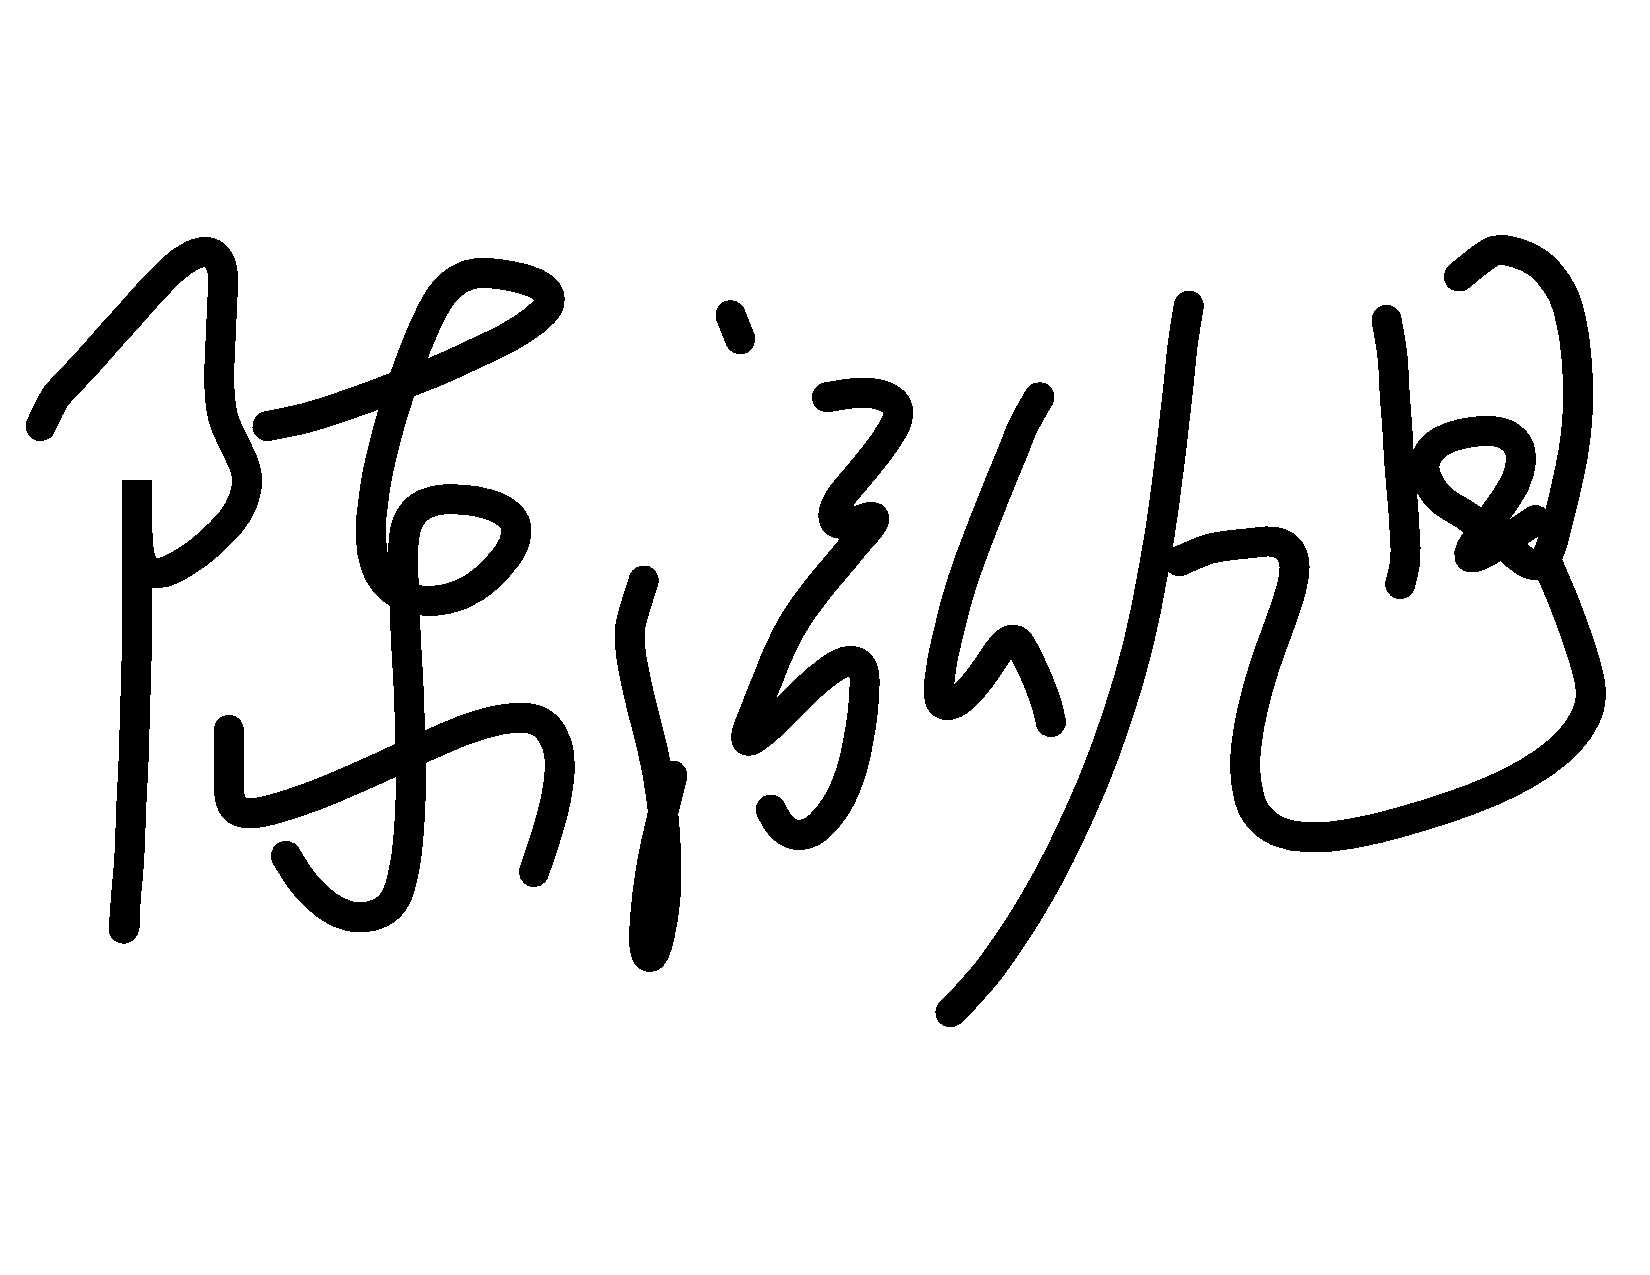
\includegraphics[width=0.09\textwidth]{res/sig_en.pdf}
\\
. . . . . . . . . . . . . . . . .\qquad \qquad \qquad \qquad\qquad \qquad . . . .  . . . . . . . . . . . . . . . . . . . . .\\
\indent \qquad Date \qquad \qquad \qquad  \qquad \qquad \qquad\qquad\qquad\qquad\qquad Hongxu Chen
